\pagenumbering{gobble}
\begin{center}
\begin{uppercase}
    {\uppercase{\fontsize{18pt}{0}\selectfont \textbf{Žilinská univerzita v Žiline} \par}}
    \vspace{5mm}
    {\uppercase{\fontsize{18pt}{0}\selectfont Fakulta riadenia a informatiky \par}}
    \vfill
        {\uppercase{\fontsize{24pt}{0}\selectfont Diplomová práca \par}}
    \vfill
\end{uppercase}
{\uppercase{\fontsize{18pt}{0}\selectfont Kristián Žuffa \par}}
\vspace{5mm}
{\fontsize{18pt}{0}\selectfont \textbf{Využitie metód umelej inteligencie pre účely} \par}
\vspace{1mm}
{\fontsize{18pt}{0}\selectfont \textbf{implementácie zvolenej aplikácie} \par}
\vspace{5mm}
Vedúci práce: Ing. Katarína Zábovská, PhD.\\
Registračné číslo: 1130/2019\\
Žilina, 2020\\
\end{center}
\pagebreak
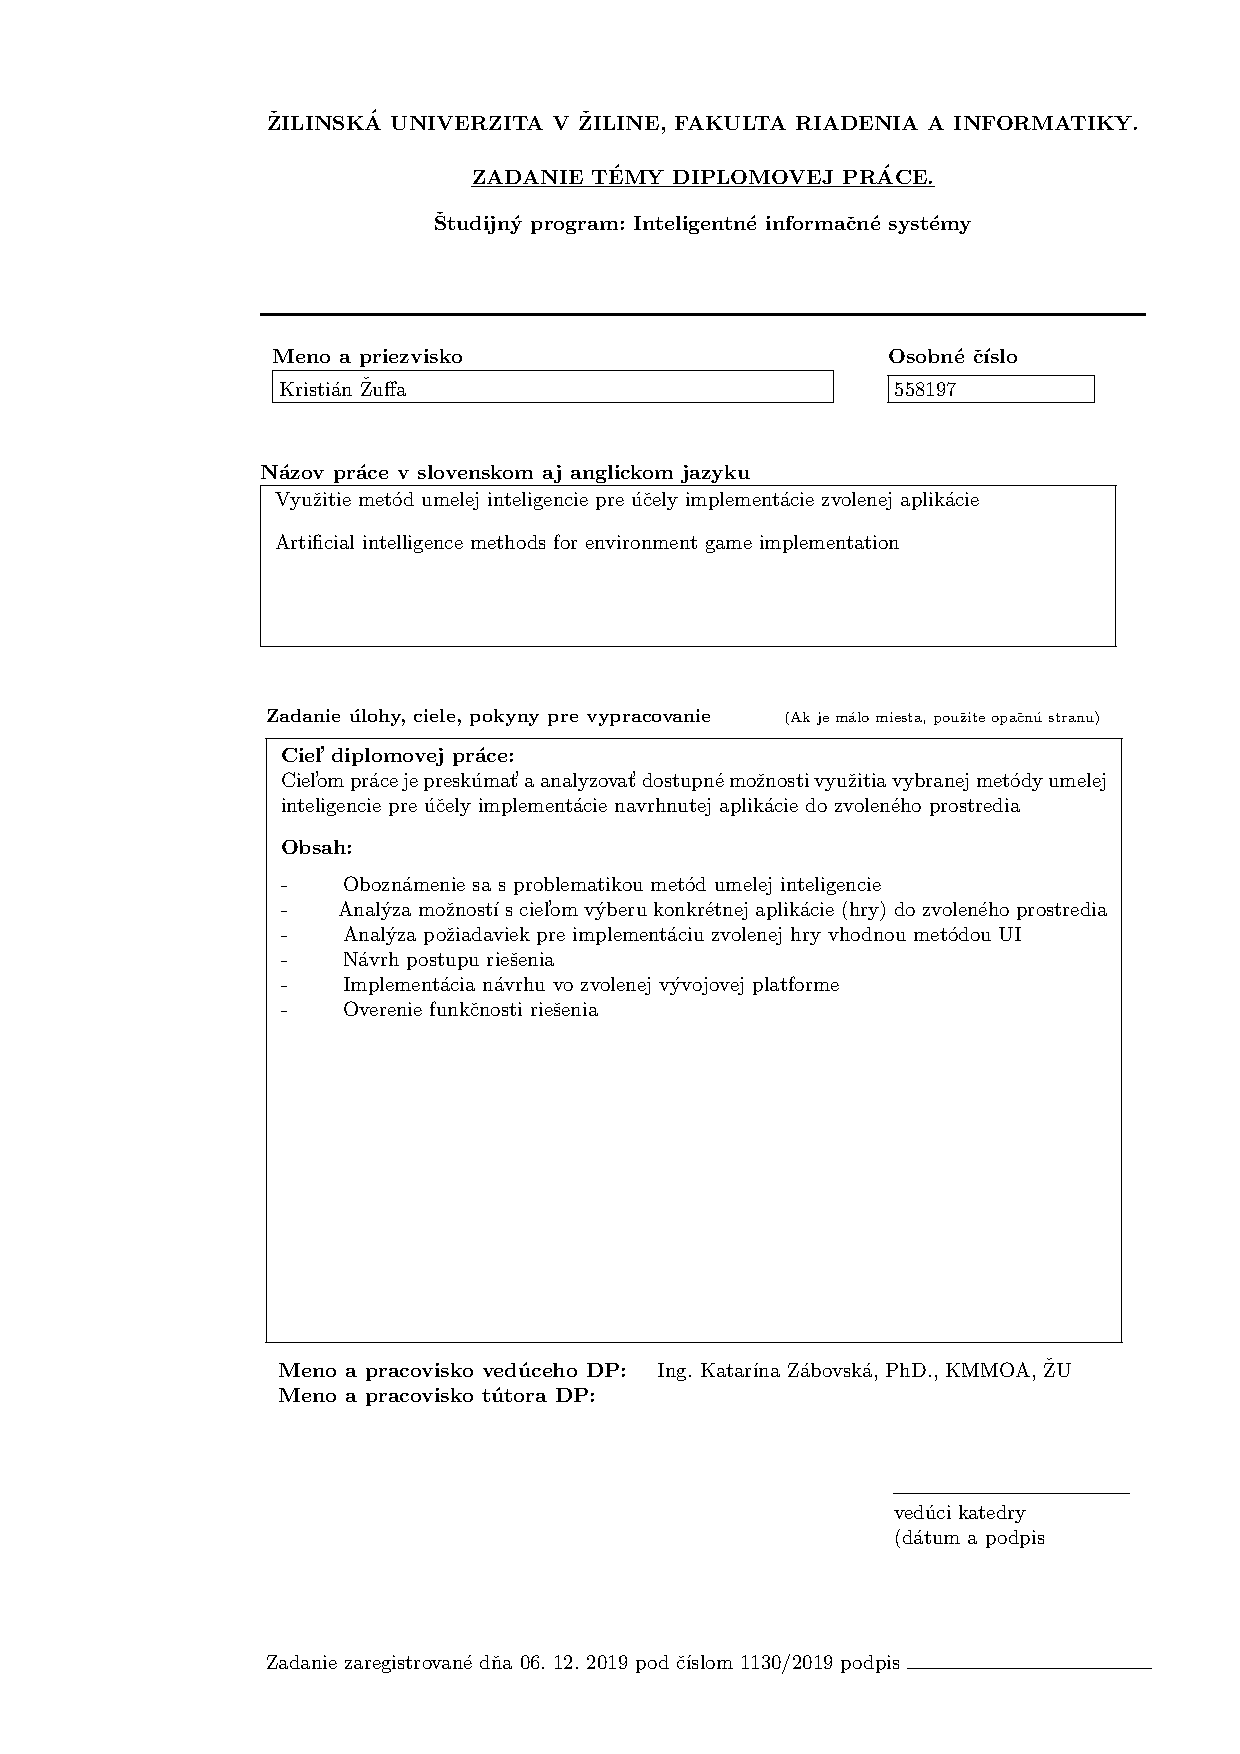
\includepdf{specification.pdf}
\pagebreak
\begin{abstract}
ŽUFFA, Kristián: Využitie metód umelej inteligencie pre účely implementácie zvolenej aplikácie do prostredia Cave.
[diplomová práca].
- Žilinská univerzita.
Fakulta riadenia a informatiky, -
Vedúci práce: Ing. Katarína Zábovská, PhD.
Stupeň odbornej kvalifikácie: inžinier.
Študijný program: inteligentné informačné systémy.
Žilina 2020.~\pageref{LastPage} strán.
\\
Táto záverečná pojednáva o analýze rôznych metód umelej inteligencie pre zvolenú konkrétnu implementáciu a to hru
piškvorky hrané v priestore (3d piškvorky).
Pri analýze boli vybraté a implementované 2 metódy: exaktná metóda minimax a umelá neurónová sieť a aplikácia bola
implementovaná do prostredia Unity.
Hra mala byť pripravená pre beh v prostredí Cave no kvôli nedostatku prostriedkov, ktorý bol spôsobený karanténou
súvisiacou s ochorením koronavírus, nebolo možné tento cieľ splniť.
Napriek tomu hra bola implementovaná ako desktopová aplikácia pre všetky komerčné platformy.
\\

ŽUFFA, Kristián: Artificial intelligence methods within the Cave environment game implementation.
[diploma thesis].
- Unifersity of Žilina.
Faculty of Management Science and Informatics, -
Supervisor: Ing. Katarína Zábovská, PhD.
Qualification: master.
Study program: intelligent information systems.
Žilina 2020.~\pageref{LastPage} pages.
\\
This thesis deals with analysis of different artificial intelligence methods for chosen specific implementation which
is the Tic-Tac-Toe game played in space (3d tic-tac-toe).
There were 2 methods analyzed and implemented: minimax exact method and artificial neural network and the game was
implemented in Unity.
The game was supposed to be ready to run in Cave environment but due to insufficient resources, caused by quarantine
related to corona virus, this target was not completed.
Despite that the game was implemented as desktop application for all commercial platforms.
\\


\end{abstract}
\tableofcontents

\listoffigures
\listoftables
\pagebreak
\pagenumbering{arabic}
\setcounter{page}{6}
